\documentclass[12pt]{article}
\usepackage[utf8]{inputenc}
\usepackage{graphicx}
\usepackage{float}
\usepackage{amsmath}
\usepackage{placeins}

\usepackage[letterpaper,margin=0.75in]{geometry}
\graphicspath{images/}
\begin{document}
\begin{titlepage}
\begin{center}
% Upper part of the page
\vbox{}
\vbox{}
\vbox{}
\vbox{}
\vbox{}
\vbox{}
\vbox{}
\vbox{}
\vbox{}
\vbox{}
\vbox{}
\vbox{}

\includegraphics[width=0.75\textwidth]{Images/ubc.png}\\[0.5cm]
\textrm{Martin Alejo}\\[0.5cm]
\catcode`#=12
\textrm{#75296665}\\[0.5cm]
\textrm{October 28, 2022}\\[0.5cm]
\textrm{Mini Project 2}\\[0.5cm]
\textrm{University of British Columbia}\\[0.5cm]
\textrm{Electrical and Computer Engineering}\\[0.5cm]
\textrm{ELEC 301}\\[0.5cm]
\textrm{Instructor: Nicolas Jaeger}\\[0.5cm]
\vbox{ }
\end{center}
\end{titlepage}
\pagebreak
\pagenumbering{roman}
\tableofcontents
\pagebreak
\listoffigures
\listoftables
\pagebreak
\pagenumbering{arabic}
\section{Introduction}
In this project, we will be using NI $Mulitsim^{TM}$ to simulate various transistors, measuring simulated values. We will also be calculating their respective theoretical values and comparing them with the simulated. We will also be assuming that $V_T=0.025V$
\section{Part 1}
\subsection{Part a)}
From the datasheet, we can see that the small signal parameters of the 2N3904 transistor for $V_{ce}= 10V, I_c = 1mA, f=1kHz,T =  25^oC$ is as follows:  

\begin{table}[h!]
\centering
\begin{tabular}{|c c c c| }
 \hline
    & Min & Max & Unit \\
    \hline\hline
$h_{fe}$ & 100 & 400 & -\\
$h_{ie}$ & 1   & 10  & k$\Omega$\\
$h_{oe}$ & 1   & 40 & $\mu mho$\\
 \hline
\end{tabular}
\caption{Small Signal Values from Data Sheet}
\label{table:small signal}
\end{table}

For this lab however, we will be using the average of those values. Therefore:
\begin{center}
$h_{fe} =250, h_{ie} = 5.5 , h_{oe} = 20.5$
\end{center}

\subsection{Part b)}

Figure \ref{fig:ibvbeib}, Figure \ref{fig:icvceib} and Figure \ref{fig:icvcevbe} below shows $I_b$ vs $V_{be}$,$I_c$ vs $V_{ce}$ and $I_c$ vs $V_{be}$ respectively.
\begin{figure}[H]
\centering
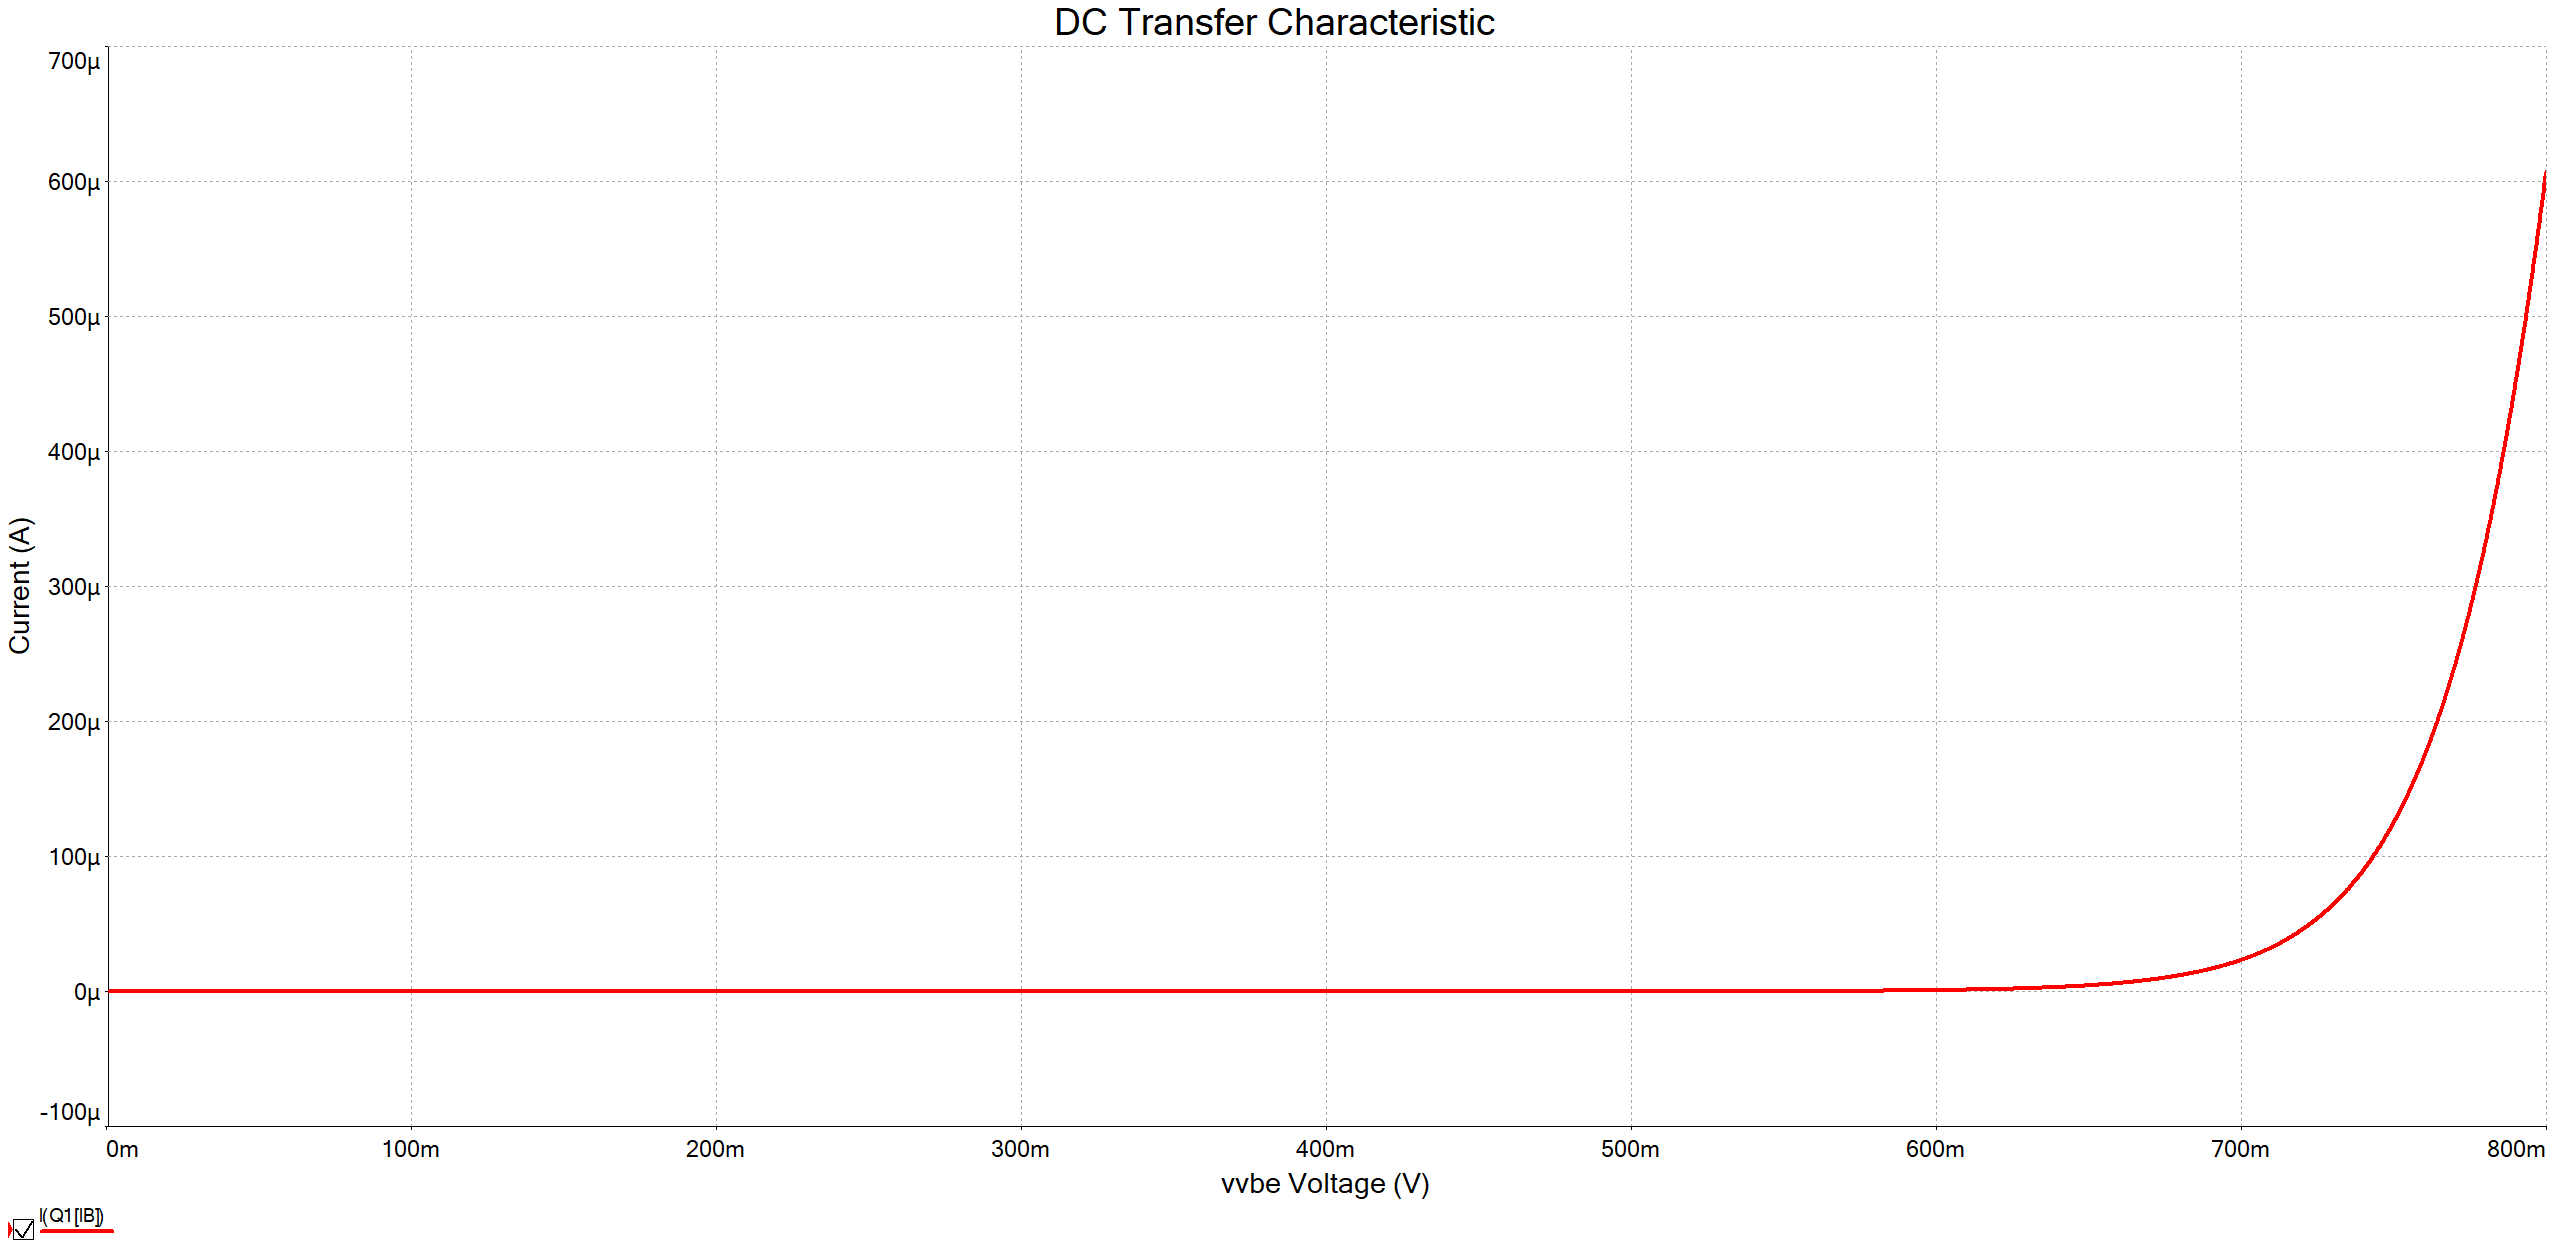
\includegraphics[width=0.75\textwidth]{Images/Ib_vs_Vbe.png}\\
\caption{$I_b$ vs $V_{be}$}
\label{fig:ibvbeib}
\end{figure}
The DC sweep of this simulation is about 0V to 2V in 0.01V increments.
\begin{figure}[H]
\centering
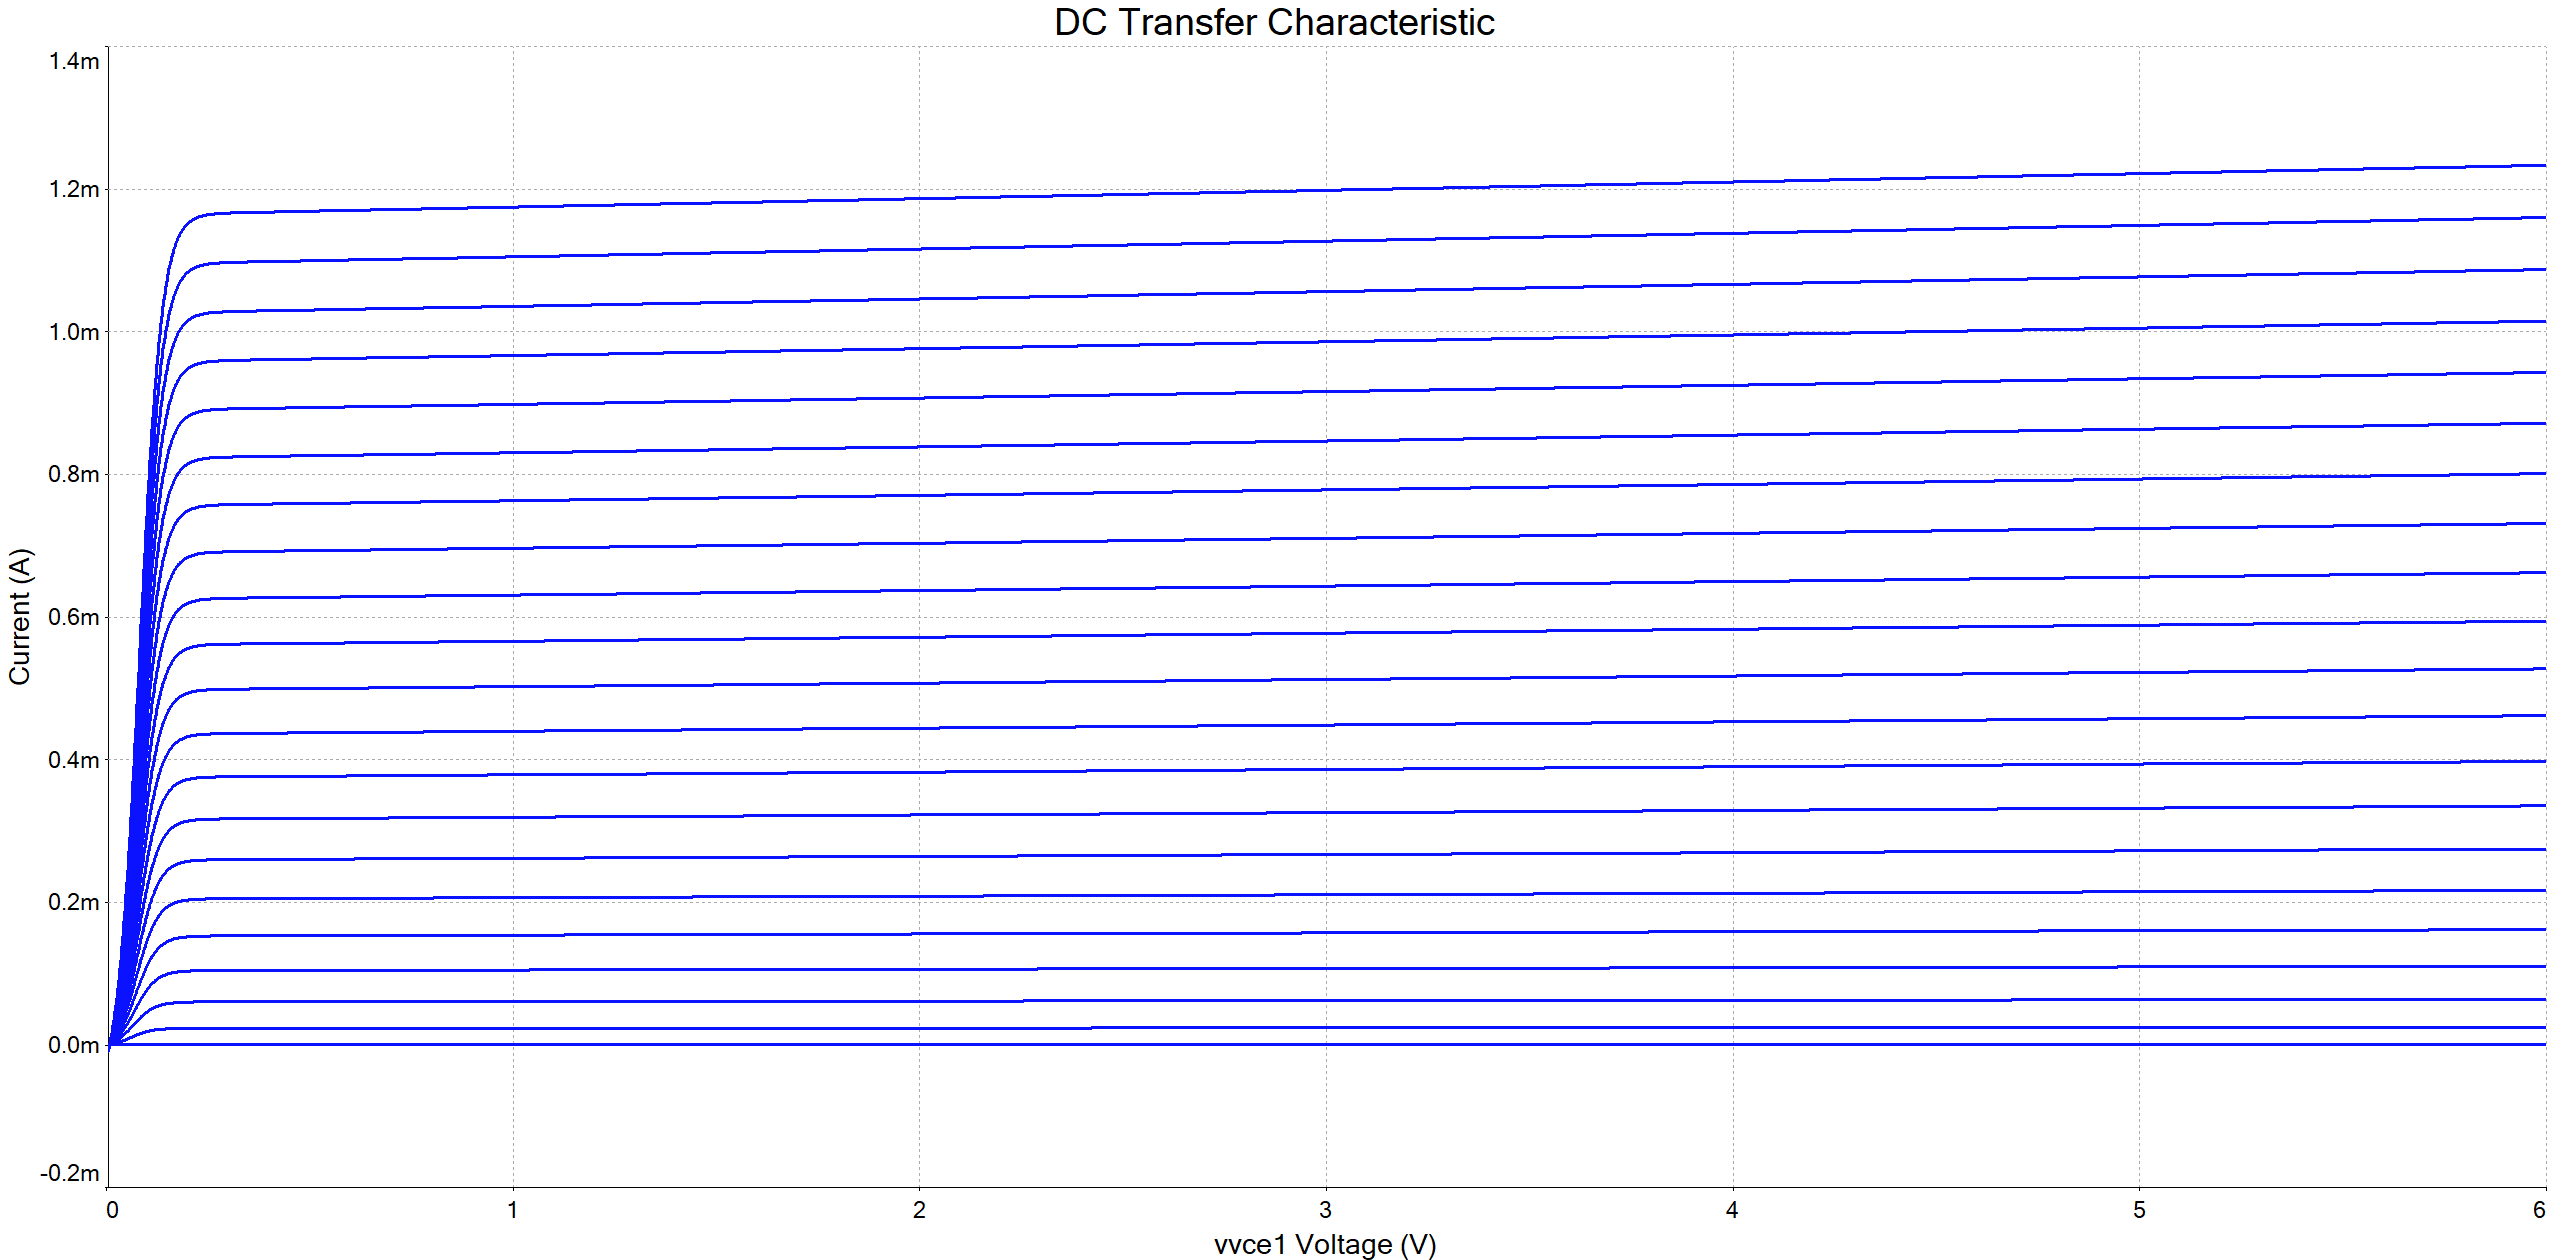
\includegraphics[width=0.75\textwidth]{Images/Ic_vs_Vce.png}\\
\caption{$I_c$ vs $V_{ce}$, varying $I_b$}
\label{fig:icvceib}
\end{figure}
The DC sweep of this simulation is $V_{ce}$ from 0 to 6V with 1mV step and $I_b$ from 0A to 10$\mu$A with $0.5\mu$A step. From this graph, we can determine the value of $I_c$ and from there, since $\beta= \frac{I_c}{I_b}$. From using the cursor tool, we can find that when $I_c=1m$A and $V_{ce}$=5V, we can see that $I_b$=$8.5\mu$A. Following the calculation that was stated previously, we can estimate that:
\newline
\begin{center}
$\beta= \frac{I_c}{I_b}$=$\frac{1*10^{-3}}{8.5*10^{-6}}$= \boxed{117}
\end{center}
\begin{figure}[H]
\centering
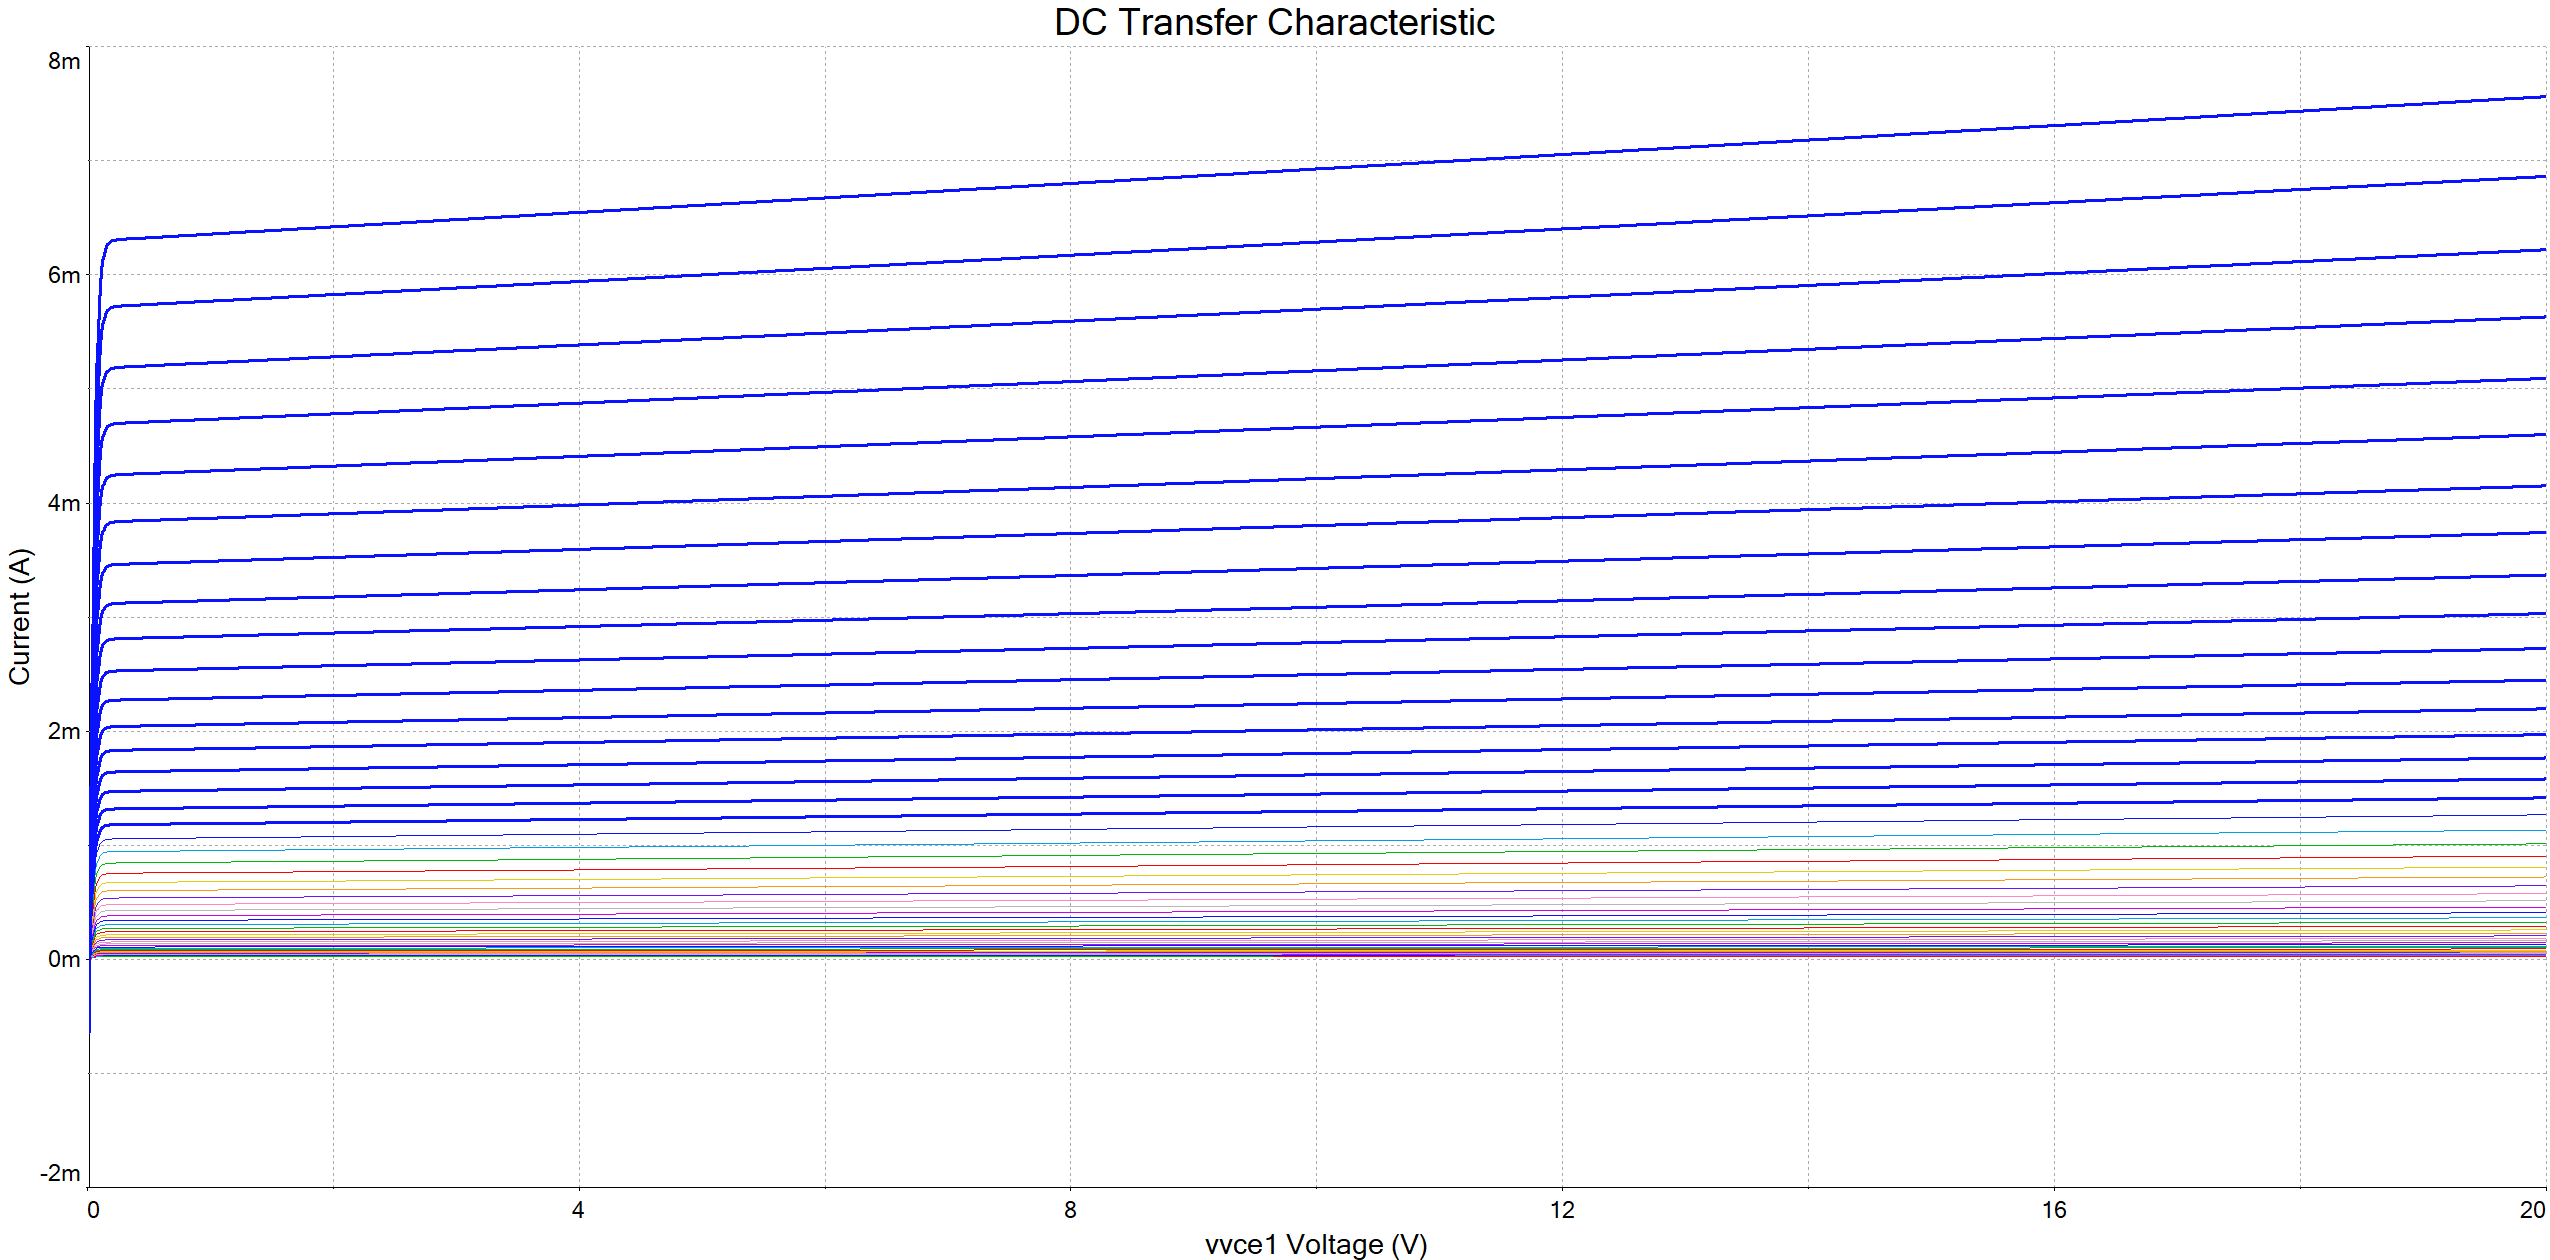
\includegraphics[width=0.75\textwidth]{Images/ic__vs_vce_vbe.png}
\caption{$I_c$ vs $V_{ce}$, varying $V_{be}$}
\label{fig:icvcevbe}
\end{figure}
The DC sweep of this simulation is $V_{ce}$ from 0 to 20V with 1mV step and $V_{be}$ from 0.55V to 0.7V with 3mA step. From the graph, when we set $V_{ce}$ = 5V and $I_c$=1mA, we can find using the cursor tool in $Multisim^{TM}$ that $V_{be}$=0.646. To find the Early Voltage ($V_A$) we can use Figure \ref{fig:icvcevbe}. Using the top-most line ($V_{be}=0.7$), we can use the slope of the linear part of that trace and find the x-intercept. The resulting x-intercept will be $V_A$. Here we can use the equation of the line to find the x-intercept, selecting two arbitrary points on that trace as $x_1$ and $y_1$:
\begin{center}
    $6.4192*10^{-3}$-y=$63.3687*10^{-6}*(x-2)$
\end{center}
setting $y=0$ and finding x, we will find that $-x=V_A$=\boxed{99.299V}
\newline
\newline
To find $r_{\pi}$, $g_m$, and $r_o$:
\begin{center}
    $r_{\pi}=\frac{\beta}{g_m}$, $g_m=\frac{I_c}{V_T}$, and $r_o =\frac{V_A}{I_c}$
\end{center}
Evaluating:
\begin{center}
 $g_m=\frac{1*10^{-3}}{0.025}$ = \boxed{0.04S},$r_{\pi}=\frac{117}{0.04}$ =\boxed{2.941k\Omega}, $r_o =\frac{99.299V}{1*10^{-3}A}$ = \boxed{99.299k\Omega}
\end{center}
\subsubsection{Comparing Values}
Comparing all of the values from the data sheet and the calculated parts, we can see that the $\beta$ value that is calculated is within the range of the minimum and maximum value as stated in the data sheet. The same can be said about the other parts that were calculated.
\subsection{Part c)}
\subsubsection{Part i)}
Finding the values of $R_{B1}$,$R_{B2}$,$R_C$,$R_E$ with:
\begin{center}
    $\beta$=117, $V_{be}=0.646V$, $I_c=1mA$, $V_{cc}=15V$,$V_{ce}=4V$, $R_E=\frac{R_C}{2}$
\end{center}

Using these values and assumptions we can find the value of $R_{C}$ assuming ($R_E=\frac{R_C}{2}$,$V_{CE}=4V$,$V_{CC}=15$) with: 
\begin{center}
$I_E=I_C+\frac{I_C}{\beta}$
\end{center}
\begin{center}
$15=I_c*R_C+4+I_E*\frac{R_C}{2}$ 
\end{center}
\begin{center}
We find that $R_C$=\boxed{7.313k\Omega}, and $R_E$=\boxed{3.656k\Omega}
\end{center}
And we can find $R_{B1}$ and $R_{B2}$ with:
\begin{center}
$\frac{15-V_B}{R_B1}=I_B+\frac{V_B}{R_{B2}}$
\end{center}
\begin{center}
$V_B=15*(\frac{R_{B2}}{R_{B1}+R_{B2}})$    
\end{center}
However, it is not possible for us to solve for $R_{B1}$, and $R_{B2}$. This is because their relationships cannot be solved with a system of linear equations. However what we can do is to estimate their values. We can choose that $R_{B1}$ is about 107k$\Omega$, and following that we can use the equations as stated previously to solve that $R_{B2}$=48.982k$\Omega$.
\subsubsection{Part ii)}
For the 1/3 rule estimation, We will be using the first version of the 1/3 rule. Where we can assume:
\begin{center}
    $V_C=V_{CC}*\frac{2}{3}$, $V_B=V_{CC}*\frac{1}{3}$,$V_{be}=0.7V$ and $I_1=\frac{I_E}{\sqrt{\beta}}$ 
\end{center}
Here is the completed circuit after finding all of the values:
\begin{figure}[H]
\centering
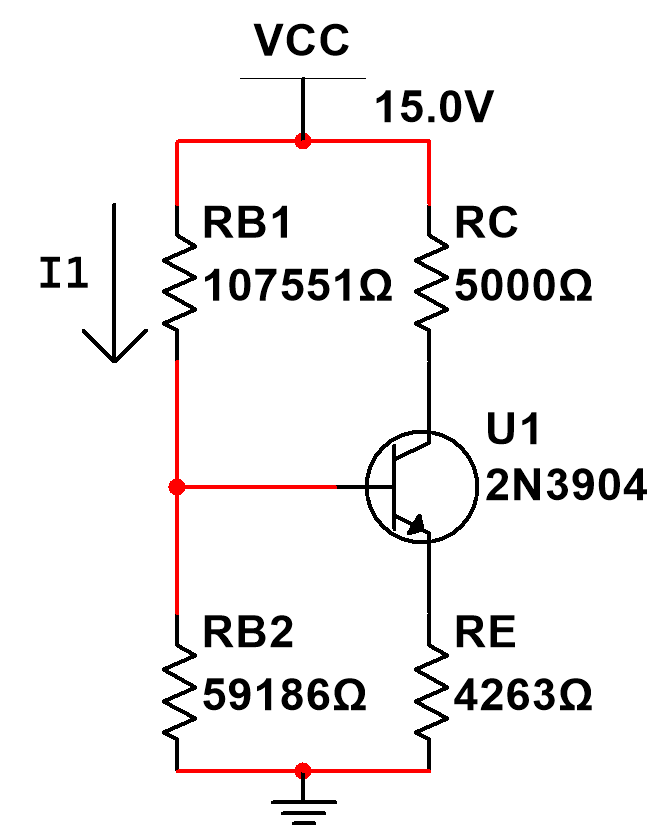
\includegraphics[height=0.25\textwidth]{Images/part1c_circuit.png}\\
\caption{Circuit With Approximated Resistor Values}
\label{fig:part1c}
\end{figure}

Here are the approximated operating points:
\begin{table}[h!]
\centering
\begin{tabular}{|l|l|l|l|l|l|}
\cline{1-6}
$I_C$      & $I_B$      & $I_E$      & $V_C$     & $V_B$     & $V_E$     \\ \cline{1-6}
\hline
1.013mA & 8.513uA & 1.021mA & 9.937V & 4.999V & 4.353V \\ 
\hline
\end{tabular}
\caption{Simulated DC Operating Point(Calculated Resistances)}
\label{table:DC Operating Values}
\end{table}
\subsubsection{Part iii)}
Here we will now design our circuit based on standard resistance values. They were chosen to be:
\begin{center}
    $R_{B1}=110k\Omega$,$R_{B2}=62k\Omega$,$R_{C}=5.1k\Omega$,$R_{E}=4.2k\Omega$
\end{center}
\begin{table}[h!]
\centering
\begin{tabular}{|l|l|l|l|l|l|}
\cline{1-6}
$I_C$      & $I_B$      & $I_E$      & $V_C$     & $V_B$     & $V_E$     \\ \cline{1-6}
\hline
1.042mA & 8.739uA & 1.051mA & 9.686V & 5.06V & 4.413V \\ 
\hline
\end{tabular}
\caption{Simulated DC Operating Point(Standard Resistances)}
\label{table:DC Standard Operating Values}
\end{table}
\subsubsection{Part iv)}
Comparing the DC operating point values from parts i),ii), and iii), we can find that the measured values with standard and calculated resistances are very similar.However, the values from Part i) are not similar to the values that we have estimated in Part ii). We can then conclude that using the $\frac{1}{3}$ rule is very accurate in estimating the resistances needed to bias the BJT.  
\subsection{Part d)}
\FloatBarrier
Here are the measured DC Operating Point values from the 2N2222A and the 2N4401 respectively:

\begin{table}[h!]
\centering
\begin{tabular}{|l|l|l|l|l|l|}
\cline{1-6}
$I_C$      & $I_B$      & $I_E$      & $V_C$     & $V_B$     & $V_E$     \\ \cline{1-6}
\hline
1.077mA & 6.409uA & 1.083mA & 9.508V & 5.153V & 4.455V \\ 
\hline
\end{tabular}
\caption{Simulated DC Operating Point(Standard Resistances, 2N2222A)}
\label{table:DC Standard Operating Values(2N2222A)}
\end{table}

\begin{table}[h!]
\centering
\begin{tabular}{|l|l|l|l|l|l|}
\cline{1-6}
$I_C$      & $I_B$      & $I_E$      & $V_C$     & $V_B$     & $V_E$     \\ \cline{1-6}
\hline
1.056mA & 7.086uA & 1.064mA & 9.612V & 5.126V & 4.467V \\ 
\hline
\end{tabular}
\caption{Simulated DC Operating Point(Standard Resistances, 2N4401)}
\label{table:DC Standard Operating Values(2N4401)}
\end{table}
\FloatBarrier
Comparing the two tables to the values from part iii), we can see that while some parts are similar, some other values are completely different. This is because of the different characteristics that each transistor has, as they are all not exactly the same.

\section{Part 2}
Here is the equivalent Common Emitter Amplifier that we will be using:

\begin{figure}[H]
\centering
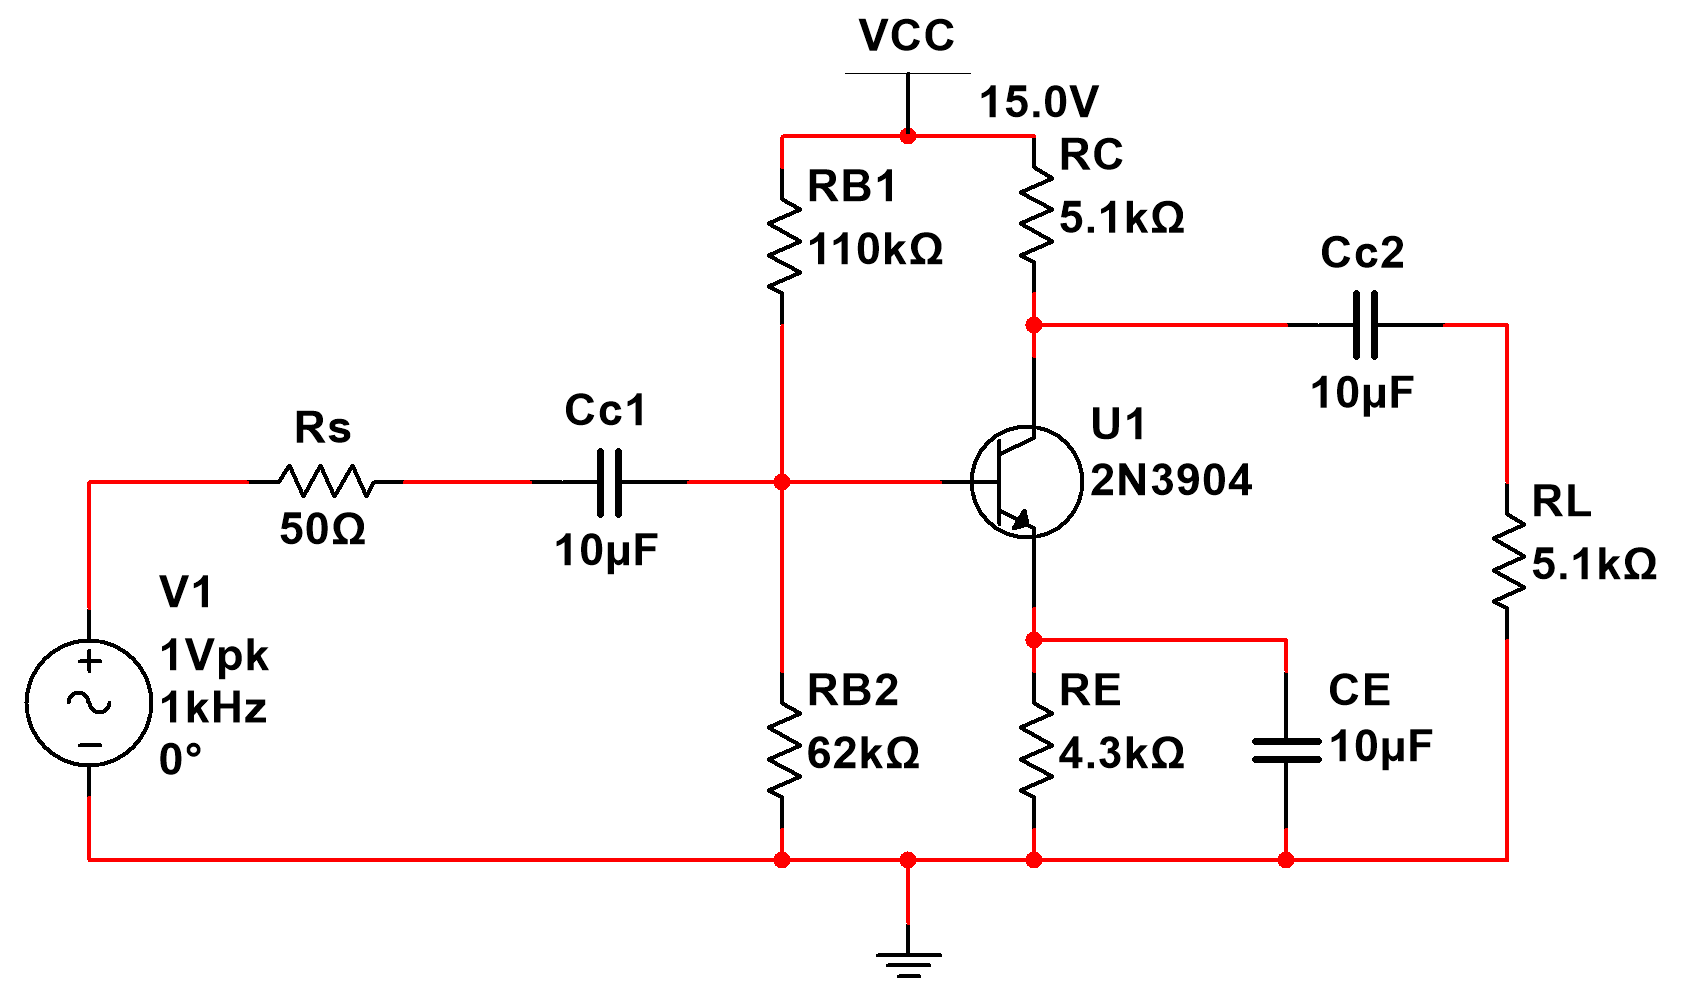
\includegraphics[height=0.30\textwidth]{Images/2acircuit.png}\\
\caption{2N3904 Common Emitter Amplifier}
\label{fig:part2a_circuit}
\end{figure}

Below is our bode plot for this circuit:

\begin{figure}[H]
\centering
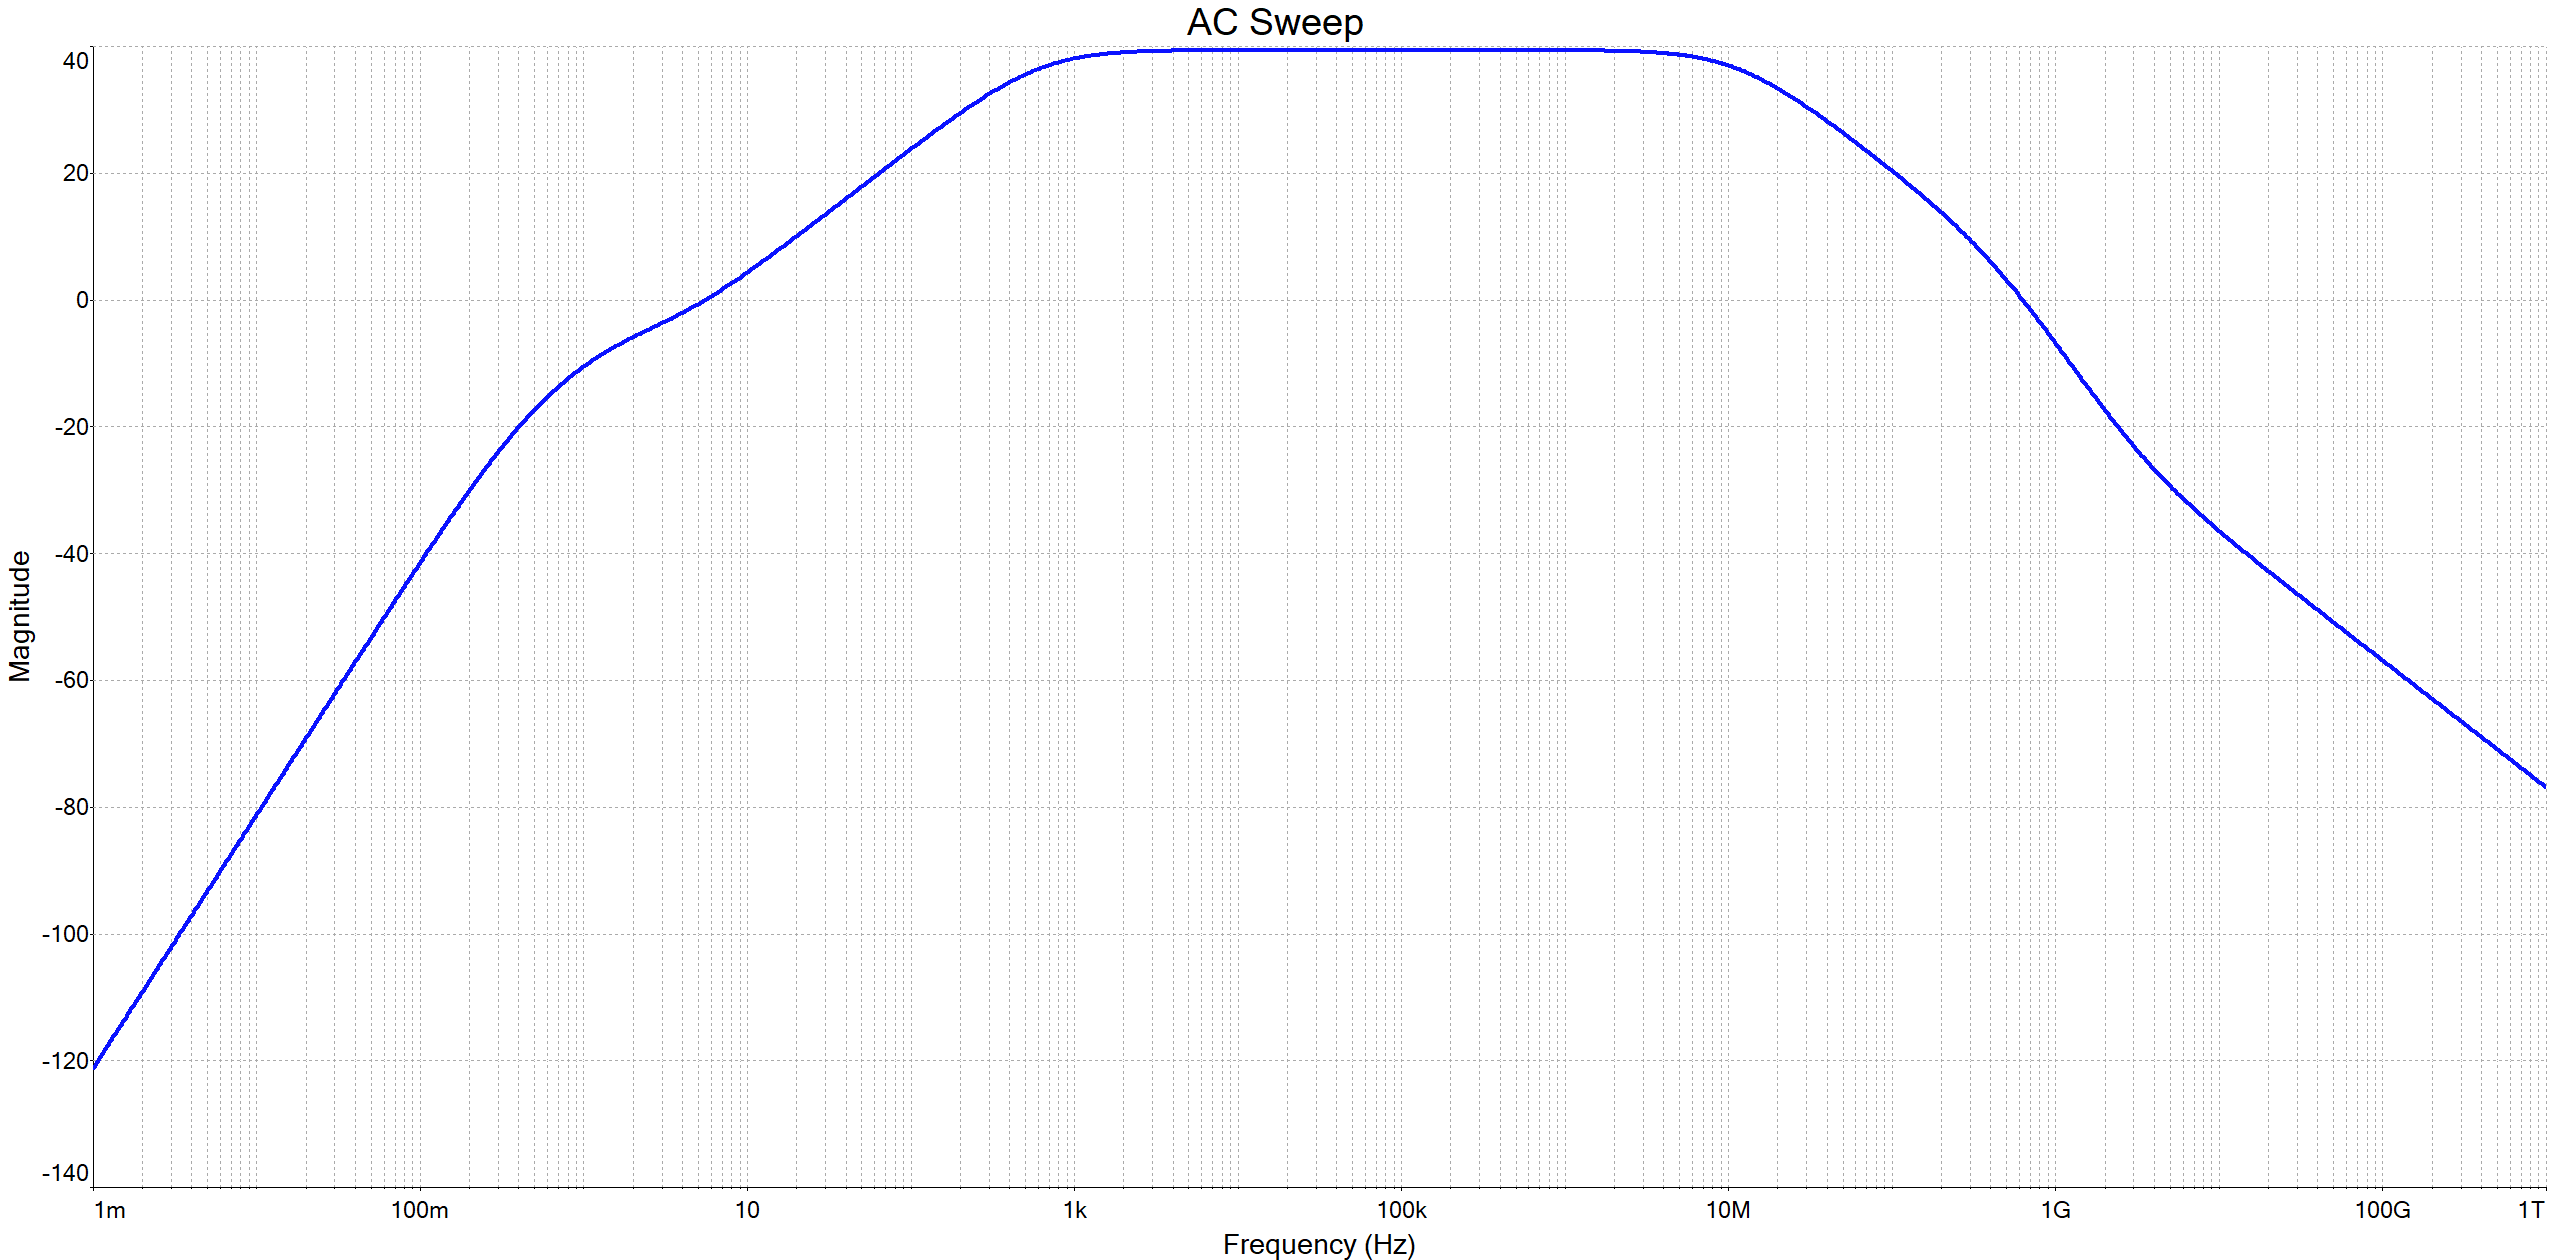
\includegraphics[height=0.35\textwidth]{Images/part2a.png}\\
\caption{2N3904 Bode Plot}
\label{fig:part2a_bodeplot}
\end{figure}
Estimating the poles, we can see where the slope changes. From there, we can use the cursor in Multisim$^{TM}$ to find the pole frequencies. Here we can see the approximated poles and zeros from Figure \ref{fig:part2a_bodeplot_approximations} below:
\begin{figure}[H]
\centering
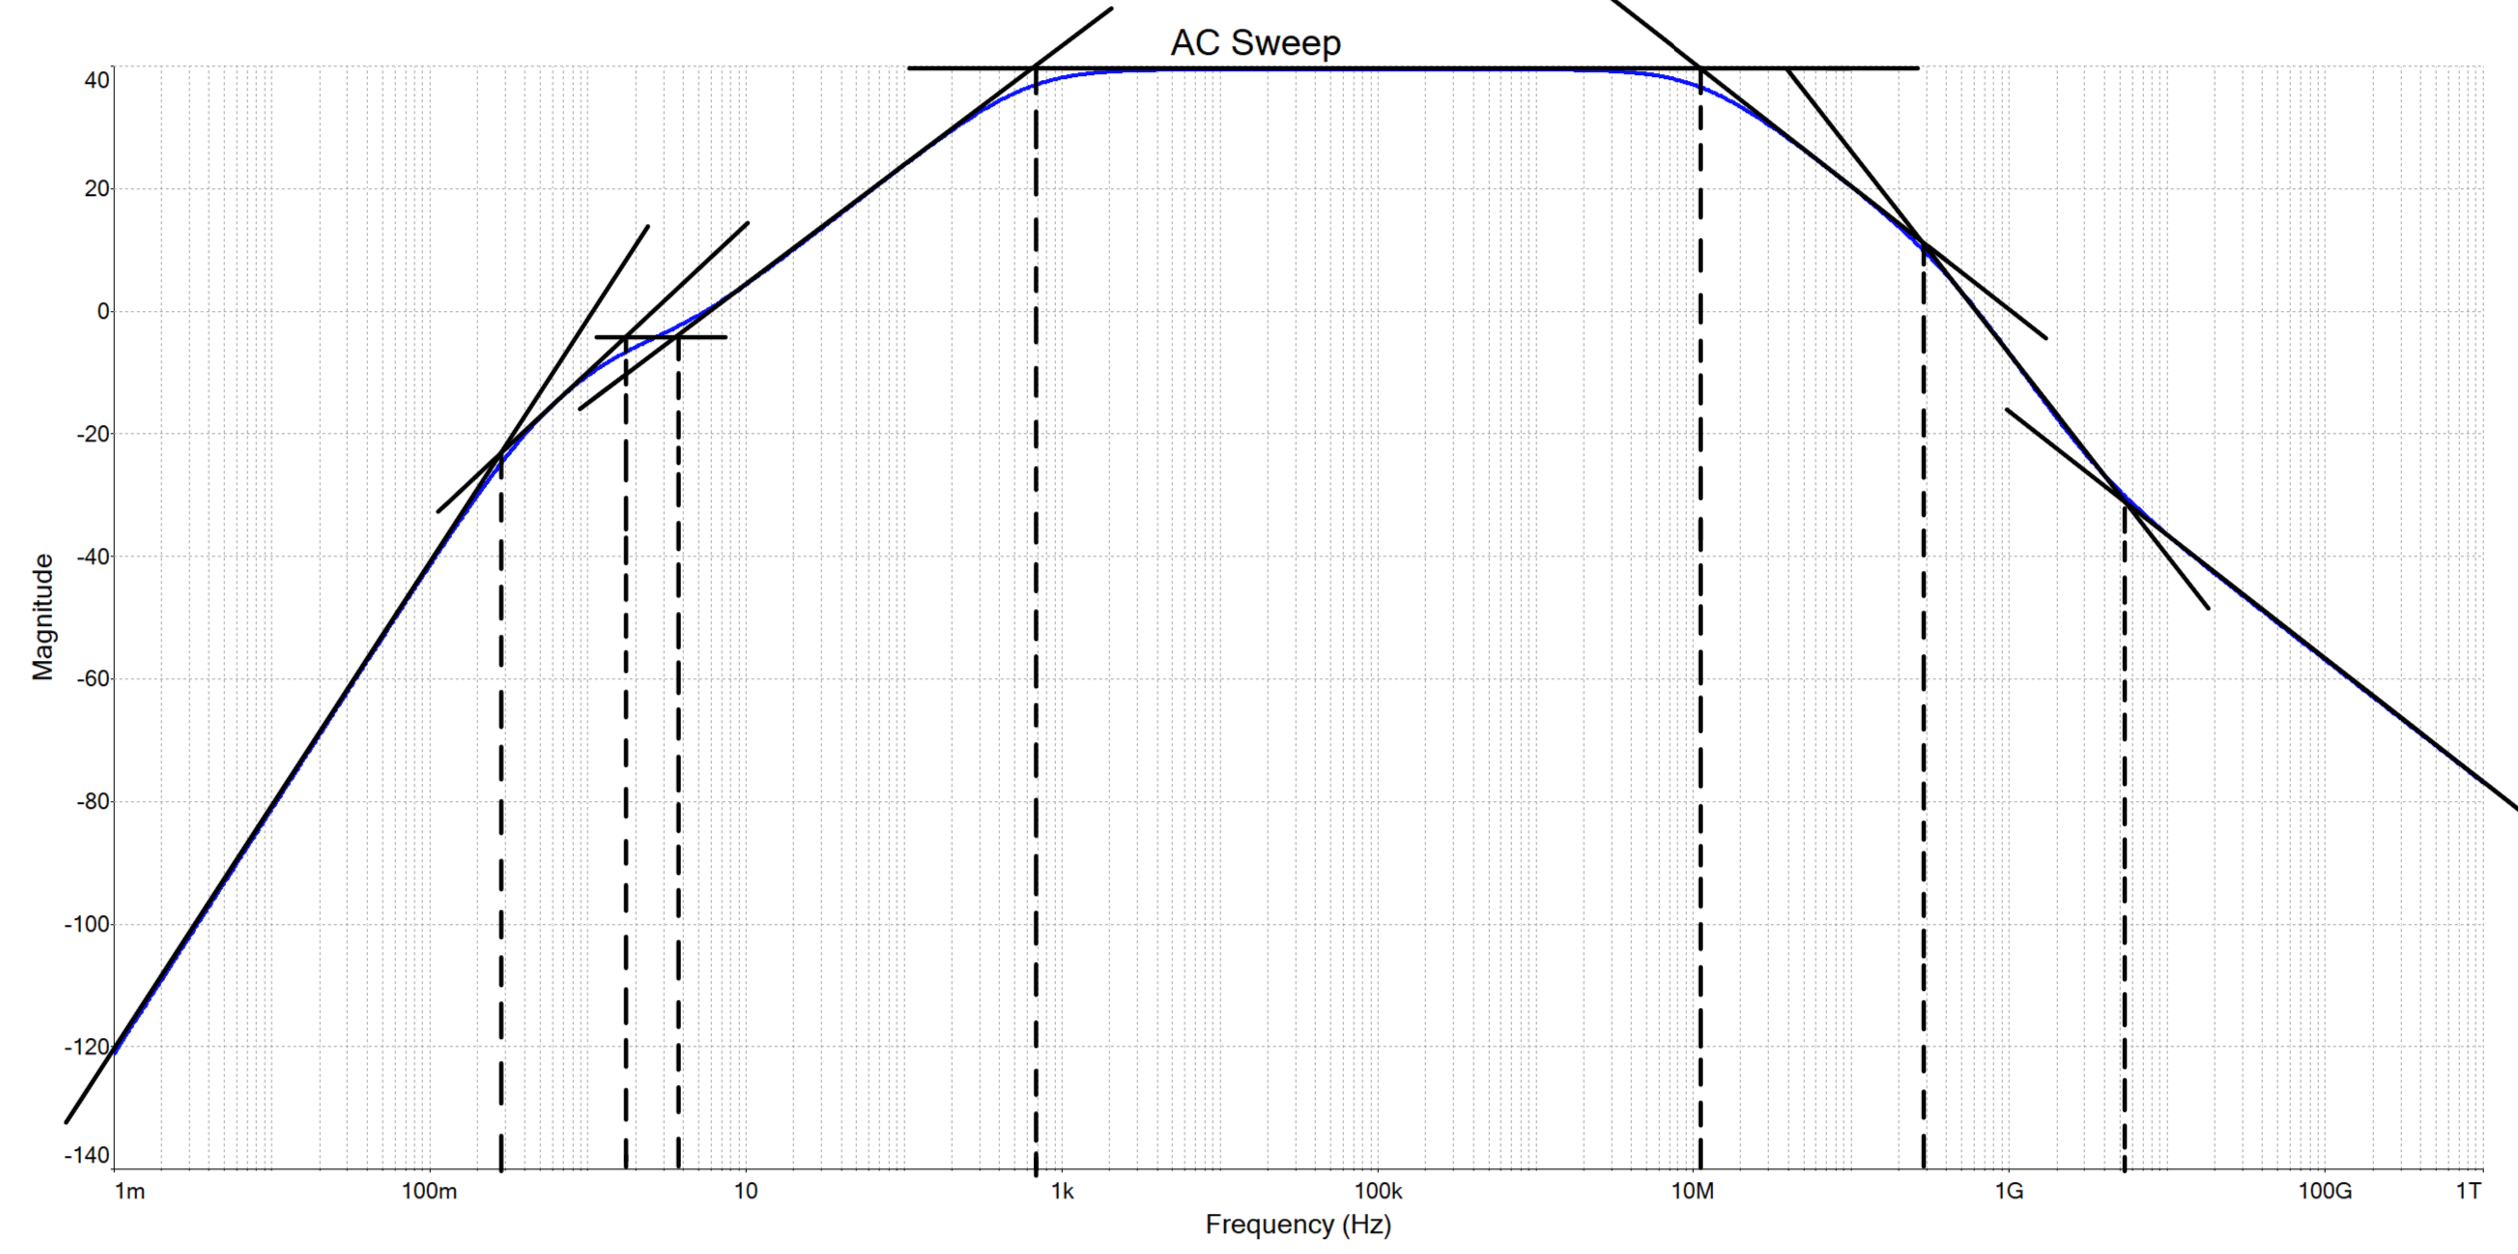
\includegraphics[height=0.35\textwidth]{Images/2abode_approximations.png}\\
\caption{2N3904 Bode Plot with Pole and Zero Approximations}
\label{fig:part2a_bodeplot_approximations}
\end{figure}
Here are the approximations:

Here are the calculations for the same transistor:




\section{Part 3}

\section{Appendix}

1. Low Frequency Circuit for Part 2 a):

\section{References}
\textrm {1. https://www.onsemi.com/pdf/datasheet/2n3903-d.pdf}\\
\textrm{2. NI Multisim Manual}\\
\textrm{3. Class Notes}\\
\end{document}
